%
% sample.tex
% $Id: sample.tex,v 1.1 2006/03/18 00:21:36 johnh Exp johnh $
%
% File is renamed to sensys-full.tex to reflect the twists made to use sensys-proc.cls.
% 

% The default of sigplan-proc-varsize is 9pt, indented paragraphs (acm style)
% For Sensys or other 10pt conference, use the 10pt option
%\documentclass{sigplan-proc-varsize}
% options:
%\documentclass[9pt]{sigplan-proc-varsize}
%\documentclass[nocopyrightspace,10pt]{sigplan-proc-varsize-sensys-abstract}

\documentclass[10pt]{sensys-proc}

% % hack to avoid the ugly ACM paragraph definition
% % => can't leave blank line after this
% (remove comment for this hack)
% \renewcommand{\paragraph}[1]{\vskip 6pt\noindent\textbf{#1 }}

\usepackage{graphicx}
\usepackage{balance}
\usepackage{comment}
\usepackage{subcaption}
\usepackage{epsfig}
\usepackage{hyperref}
\usepackage[ruled]{algorithm2e}

\numberofauthors{2}

\author{
%
% The command \alignauthor (no curly braces needed) should
% precede each author name, affiliation/snail-mail address and
% e-mail address. Additionally, tag each line of
% affiliation/address with \affaddr, and tag the
%% e-mail address with \email.
% \alignauthor Alice Security \\
%         \affaddr{Department of Computer Science}\\
%         \affaddr{University of Southern California}\\
%        \email{alice@example.edu}
% \alignauthor Bob Privacy \\
%     \affaddr{Networked Embedded Systems Group}\\
%     \affaddr{Swedish Institute of Computer Science}\\
%     \email{bob@example.se}
}

\title{Full Paper for ACM SenSys Proceedings}

\crdata{978-1-4503-1169-4}
\conferenceinfo{SenSys'13,} {November 11--15, 2013, Rome, Italy.}
\CopyrightYear{2013}

\begin{document}

\maketitle

\begin{abstract}
More than 70\% of commercial buildings have giant sensor networks to monitor different aspects of building performance. However, most of these deployed sensor networks have little metadata describing context, which precludes writing analytics applications without familiarity of the particular building’s sensor metadata structure. 

In this paper, we propose a technique which learns how to transform a building’s metadata to a common namespace by using a small number of examples from an expert. Once the transformation rules are learnt for one building, it can be applied across buildings with a similar metadata structure. We illustrate this on a testbed consisting of 60 buildings comprising more than 20,000 sensor points. We also illustrate how this common namespace can help a user write analytics applications that do not require building-specific knowledge, and also scales across different buildings. 
\end{abstract}

% A category with the (minimum) three required fields
% \category{H.4}{Information Systems Applications}{Miscellaneous}
% %A category including the fourth, optional field follows...
% \category{D.2.8}{Software Engineering}{Metrics}[complexity measures, performance measures]

% \terms{Delphi theory}

% \keywords{ACM proceedings, \LaTeX, text tagging}

\section{Introduction}

Buildings are sites of very large sensor deployments, typically containing
up to several thousand sensors reporting physical measurement, continuously.
Moreover, with the recent interest in reducing building energy consumption, it
is important to consider ways to quickly bootstrap a set of building data streams
into an anlytical pipeline to determine where there are opportunities for energy savings,
discovery of broken sensors, and assessing and tracking overall building performance.
However, current `point' naming conventions form a bottleneck in the scalability of
the data integration process.  A `point' refers to a physical location where
a sensor is taking measurements. Each building vendor uses their own naming scheme and
uniques variants of each scheme are implemented from building to building; variations exist
even across buildings that have contracted the same vendor to set up their deployment.
This makes the integration process laborious and fundamentally unscalable.  If we
wish to have a broad impact across the entire building stock, at scale, we need
to explore methods for overcoming this challenge.

Consider a simple analysis whcih has the ability
to identify anomalous readings from a specific kind of sensor.  In order to run the application
the deployer needs to know the name of the sensorand how to attain readings from it.
The stream identification process is manual.  The deployer loads the interface to the 
building management system, tracks down the spatial or system view, clicks through several windows
to locate the location of the point(s) of interest, mouses over the point(s) and records the name,
and then uses that point name to request it from the data-fetch protocol -- typically BACNet or 
LonTalk or another protocol. This process is repeated in \emph{every building} where this 
application runs.  Any application that uses building data requires access to the building
management system and the network carrying the data of interest.

In order to meaningfully deal with disparate building streams in a scalable 
fashion the streams should be \emph{searchable} across various properties, such
as building name, room location, and statistical trends.  Moreover, we
assert that wide searchability is necessary for achieving scalability.  By providing a tool for
searching across building streams, we minimize the deployment time for applications that 
allowing them to be used in \emph{all} buildings, not just a single one.  The aforementioned 
building manamgent system user interface implicitly groups sensors by location in space
or association with a system.  This grouping is also captured in the name of the point used by
the underlying communication protocol.  For example, 'AHU' -- air handling unit -- is typically
embedded in the name of every sensor that is associated with a particular air handling unit.
A similar convention is used for denoting the type of data produced by the point (i.e. all points
that contain 'ART' (area room temperature)  in their name refer to a temperature sensor).
However, these conventions vary slightly across buildings, making it difficult to
simply integrate based on such tags alone.  We need a way to unify and learn the basic
set and structure of the tags in order to unify them.

Also, commonality across certain statistical features can be used to group
different streams.  For example, consider the distribution of temperature reading across
the rooms in the building.  Given a value distribution, it might be easy to pick out values those
that classify as statistical anoamlies.  If you consider the distribution per sensor type, then
finding all statistically anomalous sensor might also identify those that are broken.
This can be determined and indexed a priori, easing the time it takes to identify the 
streams of interest to applications.

In this paper, we propose a technique which learns how to transform a building's metadata 
to a common namespace by using a small number of examples from an expert. Once the transformation 
rules are learnt for one building, it can be applied across buildings with a similar 
metadata structure.  We also show how processes that extract statistical features and generate
descriptive metadata can help unify data streams with respect to much deeper attributes.
We show how our approach makes it easier to write applications across buildings by
demonstrating its use by three different applications: 1) a rogue zone detector, 2)
a broken senor finder and 3) an application that identifies and ranks the most comfortable
rooms. We illustrate these on a testbed consisting of 60 buildings comprising more 
than 20,000 sensor points. We also illustrate how this common namespace can help a user write 
analytics applications that do not require building-specific knowledge and scales across 
different buildings. 

% We observe that every naming scheme looks to capture three point attributes: 
% 1) the location in space, 2) its relation to an subsytem, and 3) the type of 
% measurement it is taking.  

% We want to make the streams searchable.  How do we do that?
% ) We need index the metadata for the streams but the metadata available is not enough
% 2) We need to expand the metadata, but how?
% 3) name expansion --> tag unification
% 4) timeseries feature extraction --> tag unification

% top things to expand upon:  location, type, system
% secondary: statistical features about the data
 

\section{Motivation}

Buildings are notoriously complex from a management perspective.  They consume a large fraction
of the energy produced in the United States and much of is wasted~\cite{epa}.  There has been
much work in the building science community to reduce their energy consumption and make them more
efficieny, but the route to broader impact is typically carried out through regulations, guided
by the findings of studies in those communities~\cite{regulation}.
We aim to let solutions reach buildings \emph{directly} by making sense of the data they produce
as quickly and accurately as possible.
In order for this to work at scale, we must explore ways to deal with the data produced
from sensors within them and to enable braod anaysis across several buildings at a time. Our study
focuses on any building equipped with a network of sensors.  Nearly 
three-quarters of commercial buildings contain a rich sensing fabric~\cite{study}; installed as part
of their building management system.  It is the data from these system and variants of it, that
we wish to unify and make sense of in a more systematic and automated fashion.

Fortunately, we have access to a large corpus of data from buildings on our campus.
We examine the data from 56 buildings and over 22,600 points.  The maximum number of points in a 
single building is 6169 and the minimum is 27.  As expected, newer buildings have many more sense 
points than older ones -- although some old buildings that have been retrofitted have over 1000  
points. The year built for the buildings in the data set spans over 100 years -- from 1905 to 2007.
The size range is also quite broad, spanning over an order of magnitude in square footage from
about 30,000 square feet to over 360,000 square feet.

% walk through an example of point names from 2 or three buildings and explain 
% what's challenging here
%
% BLDA1R435__ART
% BLDA1R435__ARS
% BLDA1R545__ART
%Buildings consume a large fraction of the energy produced in the United States, and much of it
%is wasted\cite{epa}.  
As mentioned, buildings are notoriously complex and although many commercial 
buildings are equiped with a rich sensing infrastructure, ad-hoc data management practices
make it difficult for any analytical solution to be widely ported across building
systems.  For example, consider the following stream names: \texttt{BLDA1R435\_\_ART,
BLDA1R435\_\_ARS, BLDA1R545\_\_ART}. Each name encodes contextual information in the form
of concatinated character sequences. In these, the first 4 characters refer to the 
name of the building, the next one encodes the air handling unit association, the next 
four encode the room,
and the last three encode the acronym for the type.  Although the examples given are well
structured, many variants within the same data set exist.  For example, \texttt{BLD\_1R435\_ARG\_}
is the encoding for a different sensor in the same room as the others, but with a name
that is \emph{like} although not exactly the same structure as the others.

% Discuss how active learning technique can be used to "unify" these tag names

When dealing with a small number of points such differences are usually not a problem.  Upon 
visual inspection, the two
encodings are similar enough that the engineer can decode the meaning.  However, for automatic 
processing or processing a large number of points, these kinds of variations makes it difficult 
to generalize the character-contruction
rule set.  Without rule-set construction the data cannot be ingested properly or interpretted
correctly.  However, there are ``active learning'' techniques in the literature~\cite{ms} 
that address this problem by leveraging the knowledge of an expert. The idea behind active learning
is that you can request input from an expert to improve the accuracy of your algorithm.
In the case of name/tag expansion you 
can generalize the set of rules that generate a name/tag by example, iteratively
updating the name construction rule set for different types of names.  An expert feeds
the system examples of names for a particular type of sensor or code, and the algorithms 
that generalize the character-set construction rules can raise the confidence of the
expanded expression.
We explore the use
of \emph{active learning} techniques to iteratively learn all the variants within an across
data sets.

% expand the discussion to include sensor sin iot?


% Now discuss how the actual shapes of the readings can be quite similar looking

\begin{figure}[h!]
\centering
    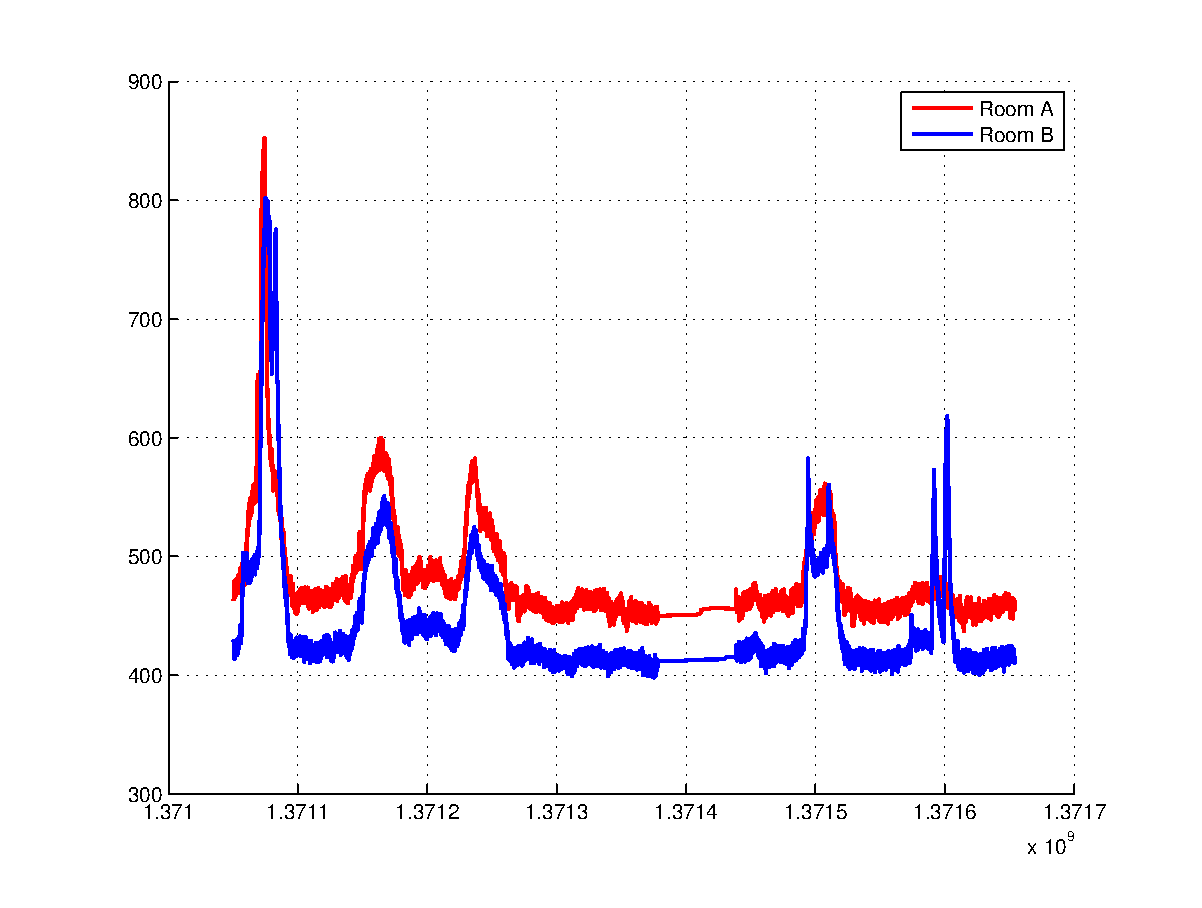
\includegraphics[width=0.48\textwidth]{figs/co2_pair.eps}
    \caption{CO2 sensor traces.}
\label{fig:co2traces}
\end{figure}

\begin{figure}[h!]
\centering
    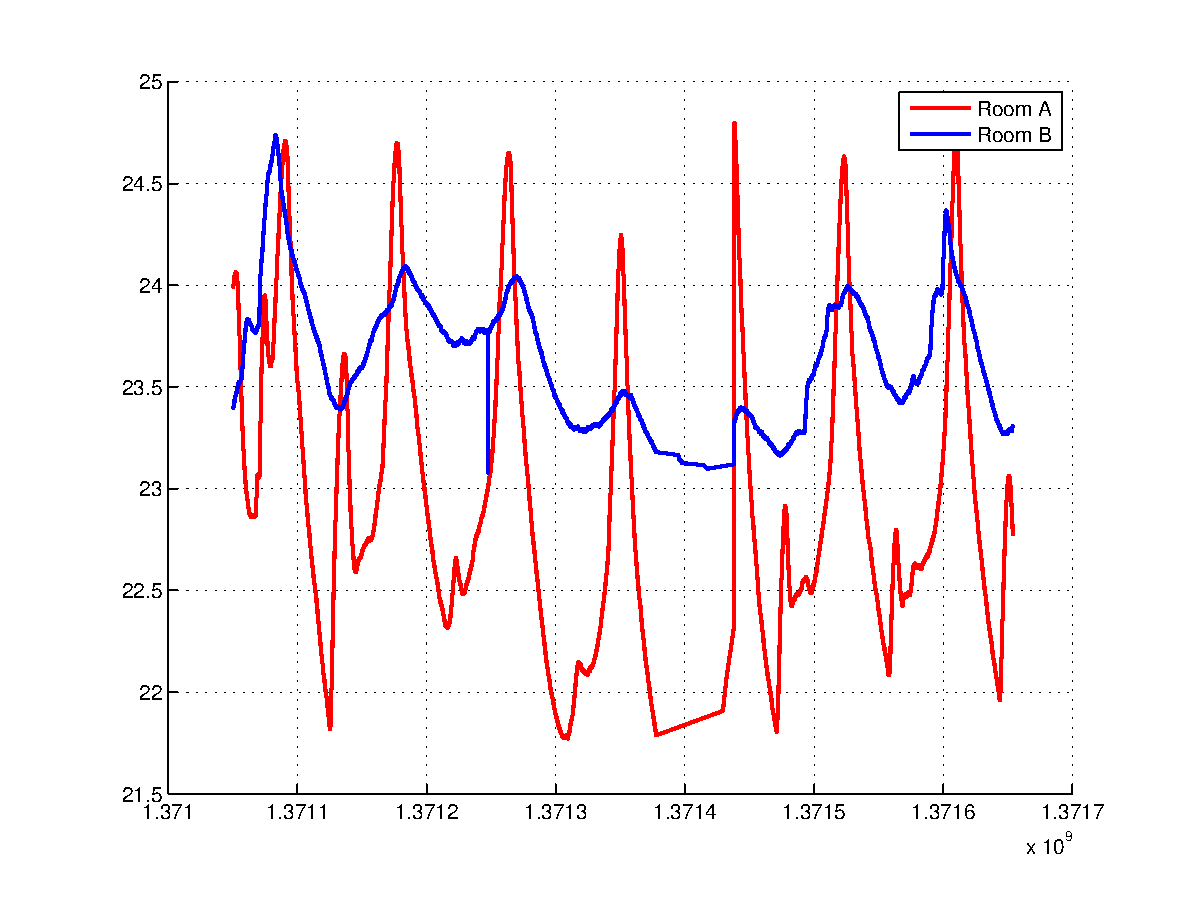
\includegraphics[width=0.48\textwidth]{figs/temp_pair.eps}
    \caption{temperature traces.}
\label{fig:temptraces}
\end{figure}

% tie this into search; search is done for scale
% scale is necessary for broad impact
% 

% discuss how both can be used to generate more metadata that we can use for indexing



\section{Related Work}

\cite{Harris:2011}
\cite{Gulwani:2011}
\cite{Singh:2012}
\cite{Gulwani12spreadsheetdata}

\section{Type Classification}
For streams with incomplete metadata that is not usable, we propose a general techique to accomplish type classification. For each stream, we use the features extracted from the readings and 


\begin{table}[h!]
%\footnotesize
 \begin{center}
	\begin{tabular}{ r|c|c|c|c|c|c|c| }
	\multicolumn{1}{r}{}
	 &  \multicolumn{1}{c}{$CO_{2}$}
	 & \multicolumn{1}{c}{$hum$}
	 & \multicolumn{1}{c}{$lum$}
	 & \multicolumn{1}{c}{$tem$}
	  & \multicolumn{1}{c}{$dvp$} 
	  & \multicolumn{1}{c}{$stp$} 
	  & \multicolumn{1}{c}{$vav$} \\
	\cline{2-8} 
	$As CO_{2}$ & 58 & 0 & 0 & 0 & 0 & 5 & 4\\
	\cline{2-8}
	$hum$ & 0 & 97 & 0 & 0 & 4 & 4 & 0\\
	\cline{2-8}
	$lum$ & 0 & 0 & 73 & 1 & 3 & 17 & 5\\
	\cline{2-8}
	$tem$ & 0 & 0 & 0 & 667 & 2 & 23 & 0\\
	\cline{2-8}
	$dvp$ & 0 & 3 & 5 & 3 & 185 & 77 & 1\\
	\cline{2-8}
	$stp$ & 5 & 7 & 14 & 24 & 46 & 1294 & 38\\
	\cline{2-8}
	$vav$ & 1 & 1 & 4 & 0 & 3 & 85 & 91\\
	\cline{2-8}
	\end{tabular}
 \end{center}
 \caption{Confusion matrix for types from all three buildings.}
 \label{tab:cluster}
\end{table}
\section{Case Study}

\begin{figure*}[ht!]
\centering
	\begin{subfigure}{0.40\textwidth}
                \centering
		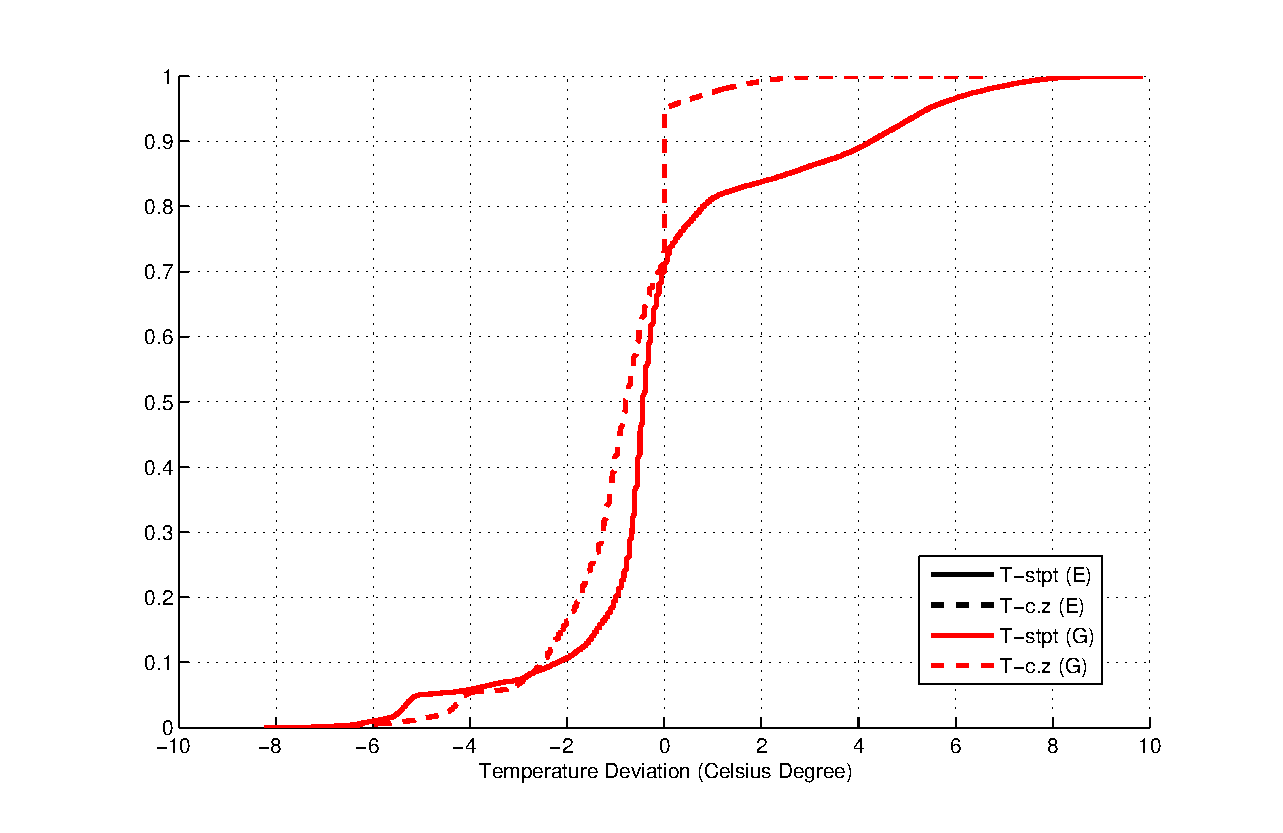
\includegraphics[width=\textwidth]{./figs/soda_cmp.eps}
                \caption{Building 1}
	\end{subfigure}
	\begin{subfigure}{0.40\textwidth}
                \centering
		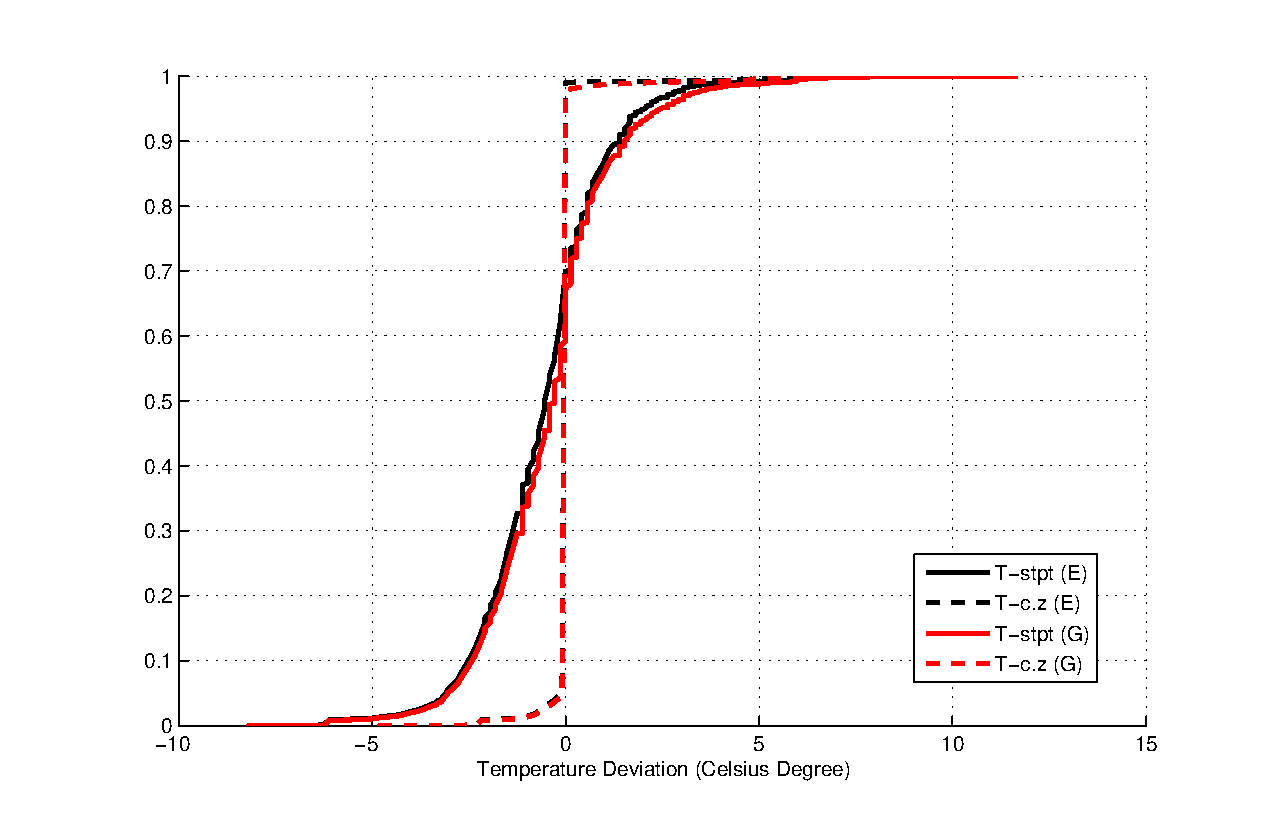
\includegraphics[width=\textwidth]{./figs/sdh_cmp.eps}
                \caption{Building 2}
	\end{subfigure}
	% \begin{subfigure}{0.32\textwidth}
 %                \centering
	% 	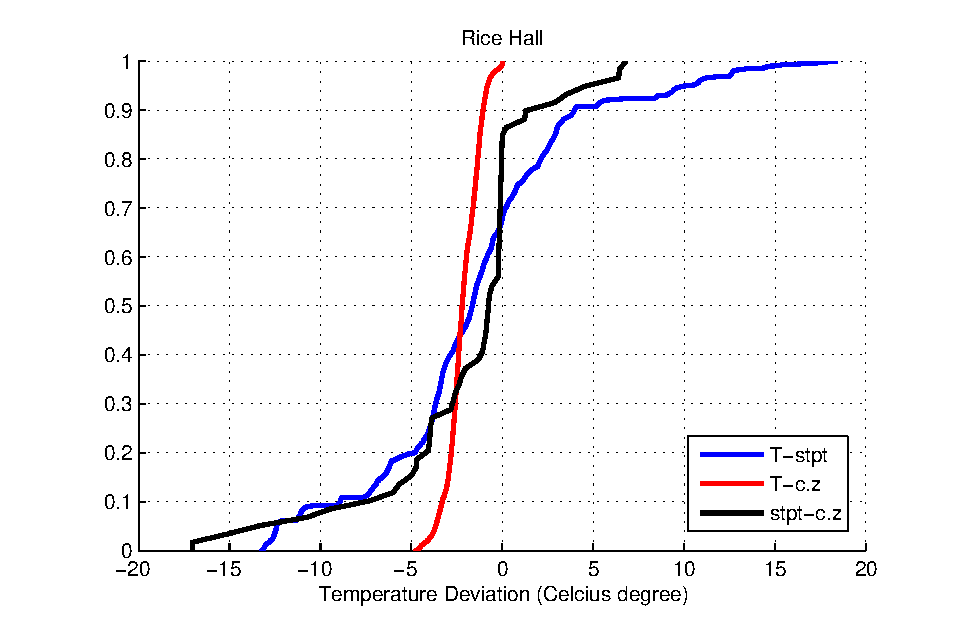
\includegraphics[width=\textwidth]{./figs/Rice_new.eps}
 %                \caption{Building C}
	% \end{subfigure}
\caption{For each building, the distribution describes the temperature deviation between: a) room temperature and the corresponding setpoint (solid), b) room temperature and the comfort range suggested by ASHRAE (dashed). The estimated distribution (labeled as ``E'') based on the expanded metadata and the ground truth distribution (labeled as ``G'') are both plotted. Note, the estimated ones overlap with the ground truth ones in the left graph.}
\label{fig:cdf_temp}
\end{figure*}

In this section, we demonstrate that with the metadata automatically expanded and normalizedusing the techniques in Section 4, we are able to implement applications that are generalizable from one building to another building without modification. As a proof of concept, we implement two applications on the two building as test bed: a) identify uncomfortable rooms and b) detect rogue rooms. We also evaluate the metadata expansion technique in terms of the accuracy for both applications compared against the ground truth. 

\subsection{Experimental Setup}
We implement two applications and perform the analysis on the same two buildings used in Section 5.1, and each building is installed with a different management system. Building 1 uses the system from Barrington while building 2 is installed with the Siemens BACnet system~\cite{bacnet}. We used the temperature data as well as setpoint information of the rooms in each building. The temperature measurements are reported every 15 seconds and the data used for analysis is from one week in June 2009 and January 2012 respectively. Particularly, we pick the data during the working hours from 9am to 5pm for analysis.

\subsection{Uncomfortable Rooms}
It's not unusual to have rooms in a building stay extremely cold or hot thus making the occupants feel uncomfortable and incurring energy waste. The discomfort is usually caused by improper setpoint configuration or dysfunction of the HVAC systems, and being able to identify these uncomfortable zones or rooms in the building is vital to improve occupant comfort as well as achieve potential energy savings. With the metadata normalized using our techniques, we are able to search for the desired streams, e.g., the temperature and setpoint of a room, and analyze the thermal performance of different buildings despite of the different naming schema used to label sensors and meters.

To identify the discomfort in a building, for each room we are particularly interested in 1) how much does the temperature deviate from the comfort range? 2) how much does the temperature deviate from the setpoint? To answer both questions, we first search through the points in each building for distinct temperature stream of each room and the corresponding setpoint. Then we compare the temperature with the setpoint as well as the suggested comfort range by ASHRAE (73F-81F for summer and 67F-76F for winter) to compute the temperature deviations from the aforementioned three different perspectives in one-week period. We accumulate the results from all the rooms per building and generate the distribution as illustrated in Figure~\ref{fig:cdf_temp}.

Figure~\ref{fig:cdf_temp} presents the temperature deviation distribution for both buildings where the results are generated from the expanded metadata following the above steps. We also present the ground truth of temperature deviation distribution, where we manually find the temperature and setpoint streams for all rooms. Each graph shows how much the temperature of a building deviates from the setpoint (solid) and the comfort range (dashed). On average, both buildings are uncomfortable to some degree and to better understand which dominant rooms are uncomfortable, and the estimated distributions using expanded metadata are close to the ground truth ones. To gain further insight, we rank the rooms in each building by how much time they deviate from the comfort zone and the ranking results are shown in Table~\ref{tab:uncmft}.

\begin{table}[h]
%\footnotesize
 \begin{center}
	\begin{tabular}{|c|c|c|c|}
	\multicolumn{2}{c}{$Bldg 1$}
	 & \multicolumn{2}{c}{$Bldg 2$}\\
	\cline{1-4} 
	 room\# & \% & room\# & \%\\
	\cline{1-4}
	 326 & 1 & 330B & 1\\
	\cline{1-4}
	 340 & 1 & 213 & 1\\
	\cline{1-4}
	352 & 1 & 148 & 0.72\\
	\cline{1-4}
	364 & 1 & 629 & 0.54\\
	\cline{1-4}
	376A & 1 & 768 & 0.49\\
	\cline{1-4}
	380 & 1 & 458 & 0.45\\
	\cline{1-4}
	384 & 1 & 621 & 0.44\\
	\cline{1-4}
	405A & 1 & 750 & 0.42\\
	\cline{1-4}
	405B & 1 & 571 & 0.35\\
	\cline{1-4}
	410A & 1 & 548 & 0.29\\
	\cline{1-4}
	\end{tabular}
 \end{center}
 \caption{Ground truth for how much time each room's temperature is outside the comfort range: rooms in each buidling are ranked by how much time they are uncomfortable throughout the one week period, and the first ten rooms on the ranking of each building are listed.}
 \label{tab:uncmft}
\end{table}

Moreover, for building 1 we group the identified uncomfortable rooms down to their corresponding air handler units (AHU), as shown in Figure~\ref{fig:soda_zone1}. For each AHU zone, we present the number of rooms in it, the number of rooms whose temperature have been at least once outside the comfort range thus being uncomfortable, and , the number of rooms that have been uncomfortable in more than 50\% of the one-week time. We see that for each AHU zone a large portion of the rooms are uncomfortable in even more than 50\% of the time, indicating the building was very likely to operate under a improper schedule. The ground truth analysis covers all the rooms in each building, so all potential uncomfortable rooms are identified here. However, the analysis using the name points expanded with our techniques would miss some of the uncomfortable rooms because the expansion contains certain error rates. We will discuss the error rates later.

\begin{figure*}[ht!]
\centering
	\begin{subfigure}{0.48\textwidth}
                \centering
		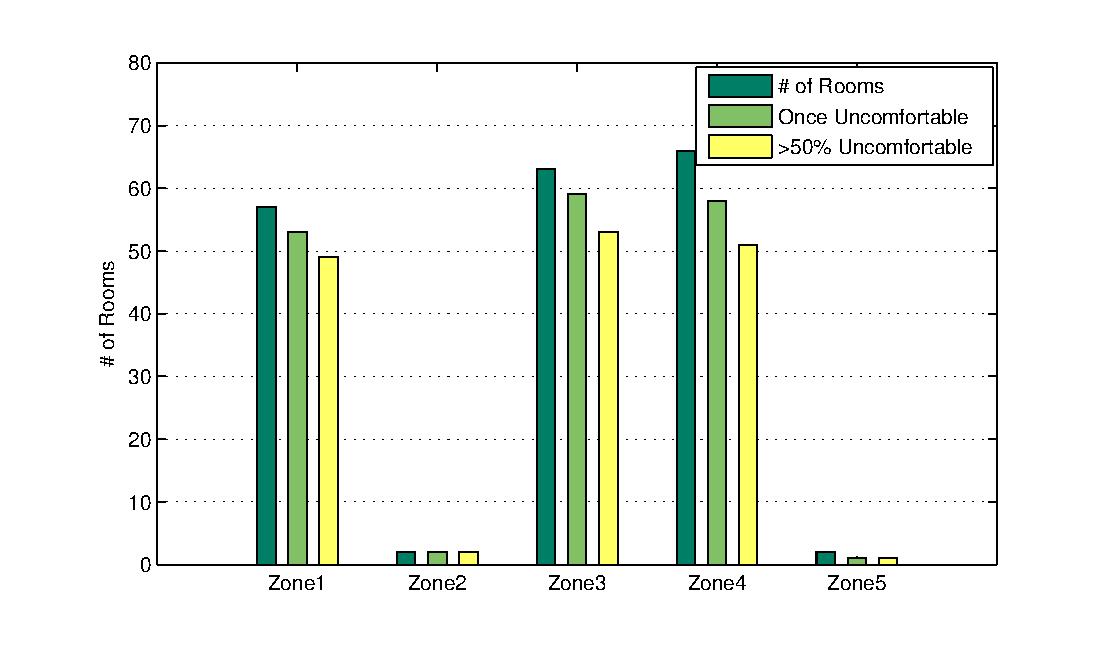
\includegraphics[width=\textwidth]{./figs/uncmft_soda.eps}
                \caption{Uncomfortable Rooms}
                \label{fig:soda_zone1}
	\end{subfigure}
	\begin{subfigure}{0.48\textwidth}
                \centering
		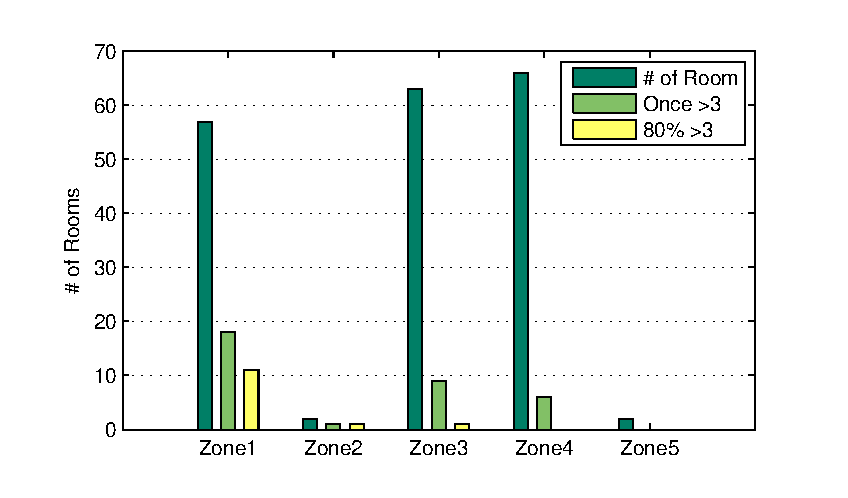
\includegraphics[width=\textwidth]{./figs/rogue_soda.eps}
                \caption{Rogue Rooms}
                \label{fig:soda_zone2}

	\end{subfigure}
\caption{Breakdown of the uncomfortable and rogue rooms in building 1 by air handler unit zone. Uncomfortable rooms are those whose temperature at least once exceeds the comfort range suggested by ASHRAE. Rogue rooms are those whose temperature deviates from the setpoint more than 3 Celsius degree. For each zone, we show the number of rooms in it, the number of zones at least once meets the criterion, and the number of rooms that meet the criterion in more than 50\%/80\% of the one-week period.}
\end{figure*}

\subsection{Rogue Rooms}
Heating and cooling contribute to the largest portion of energy consumption of a building, and often, HVAC system operates abnormally either because the system fails itself or the schedule of the building is problematic. And there are often some zones and rooms in a building that are constantly cold or hot than the neighbors thus incurring energy waste. We demonstrated the temperature deviation distribution above, and we are particularly interested in the periods when a room deviates from the setpoint more than 3 Celsius degree, which indicates that the room is highly likely to be under either heating or cooling. Therefore, for each building, using this criterion, we zoom in to the interested portion on the temperature deviation distribution and find rooms falling into this portion in most of the time. The ground truth results are summarized in Table~\ref{tab:rogue}. Again, we group the rooms according to their air handler unit ID and show the results in Figure~\ref{fig:soda_zone2}. We see that there are 13 rogues rooms all together in building 1, and 11 of them belong to AHU1, suggesting the unit might be either wrongly configured or misoperating.

\begin{table}[h!]
%\footnotesize
 \begin{center}
	\begin{tabular}{|c|c|c|c|}
	\multicolumn{2}{c}{$Bldg 1$}
	 & \multicolumn{2}{c}{$Bldg 2$}\\
	\cline{1-4} 
	 room\# & \% & room\# & \%\\
	\cline{1-4}
	 330B & 1 & 330B & 1\\
	\cline{1-4}
	 340 & 1 & 213 & 1\\
	\cline{1-4}
	420A & 1 & 148 & 0.93\\
	\cline{1-4}
	420 & 1 & 768 & 0.67\\
	\cline{1-4}
	698 & 1 & 371 & 0.62\\
	\cline{1-4}
	442 & 0.996 & 458 & 0.62\\
	\cline{1-4}
	398 & 0.981 & 538 & 0.57\\
	\cline{1-4}
	336 & 0.96 & 413 & 0.54\\
	\cline{1-4}
	183 & 0.92 & 558 & 0.48\\
	\cline{1-4}
	498 & 0.91 & 548 & 0.47\\
	\cline{1-4}
	\end{tabular}
 \end{center}
 \caption{Ground truth for how much time each room's temperature deviates from the setpoint more than 3 Celsius degree. For each building, the first column is room number and the second column is the percentage of the one-week time that the room deviates that much. The first ten rooms on the ranking of each building are listed.}
 \label{tab:rogue}
\end{table}

% \begin{figure*}[h!]
% \centering
% 	\begin{subfigure}{0.48\textwidth}
%                 \centering
% 		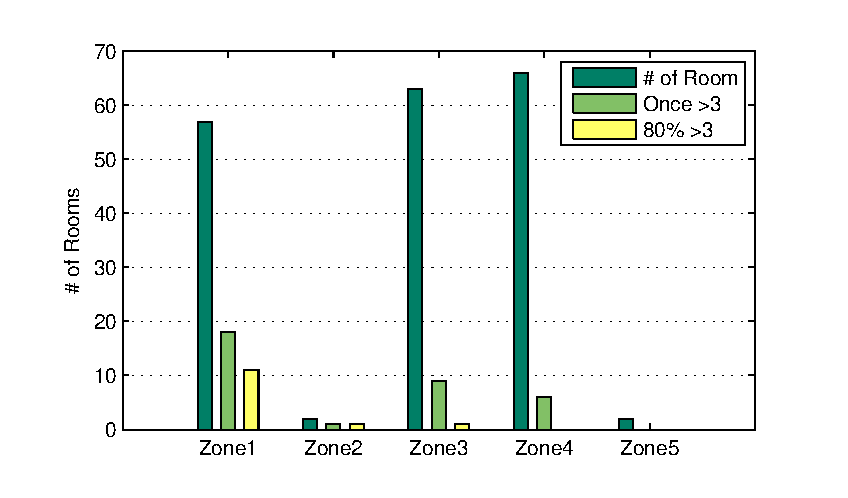
\includegraphics[width=\textwidth]{./figs/rogue_soda.eps}
%                 \caption{Building A}
% 	\end{subfigure}
% 	\begin{subfigure}{0.48\textwidth}
%                 \centering
% 		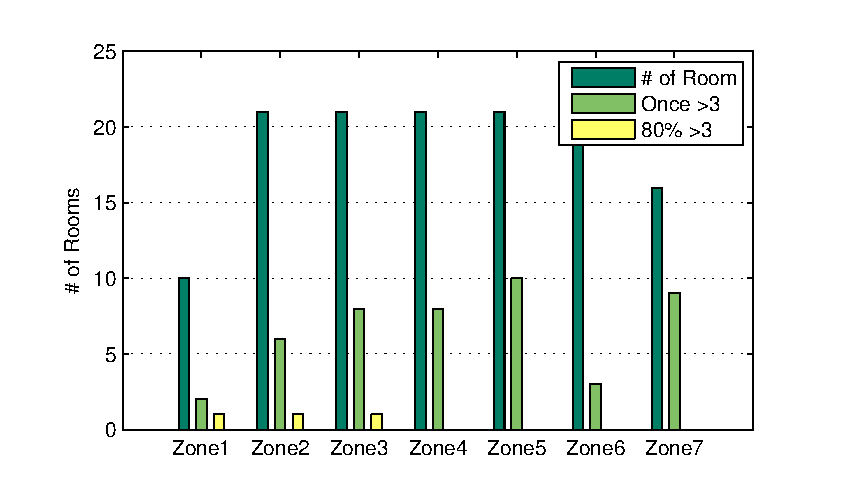
\includegraphics[width=\textwidth]{./figs/rogue_sdh.eps}
%                 \caption{Building B}
% 	\end{subfigure}
% \caption{Dividing the rooms whose temperature once deviates from the setpoint more than 3 Celsius degree by HVAC zones: for each zone, we show the number of rooms in the zone, the number of zones once appears to be rogue, and the number of rooms that were rogues more than 80\% in the one-week period.} 
% \label{fig:rogue}
% \end{figure*}

\begin{figure*}[ht!]
\centering
	\begin{subfigure}{0.48\textwidth}
                \centering
		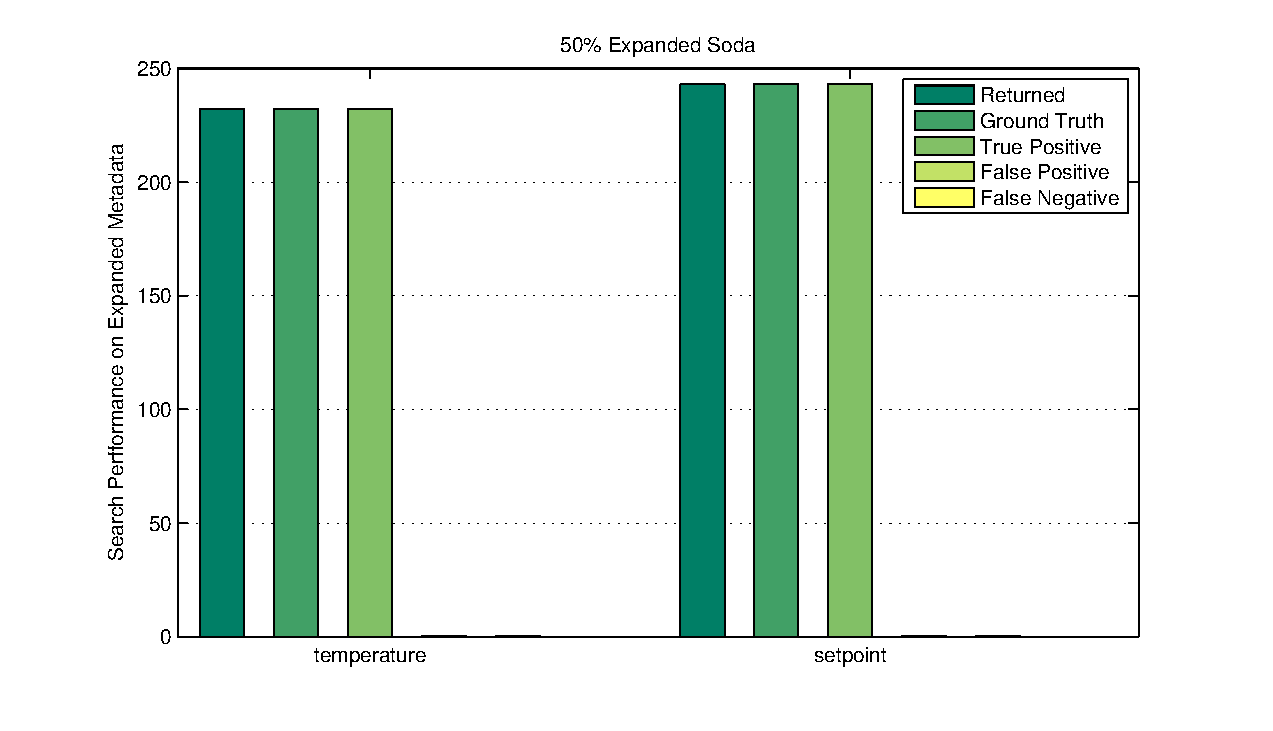
\includegraphics[width=\textwidth]{./figs/50-soda.eps}
                \caption{Building 1}
	\end{subfigure}
	\begin{subfigure}{0.48\textwidth}
                \centering
		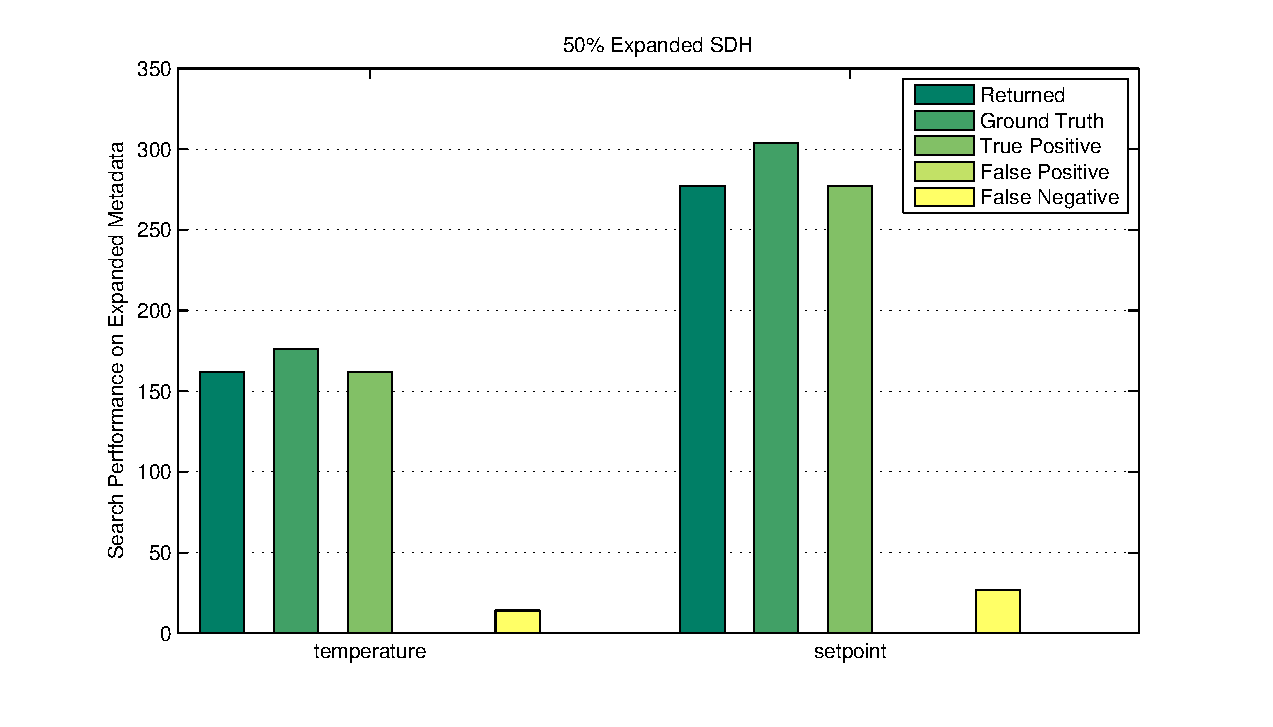
\includegraphics[width=\textwidth]{./figs/50-sdh.eps}
                \caption{Building 2}
	\end{subfigure}
\caption{The error rates of searches over the expanded metadata using our techniques. Two searches are performed particularly: ``room temp'' and ``room temp setpoint''.}
\label{fig:error}
\end{figure*}

%156,0,8; 13,0,3; 4,0,0; 3,0,3
\begin{table}[h!]
%\footnotesize
 \begin{center}
\begin{tabular}{rcc}
\multicolumn{1}{l}{} & Bldg 1                 & Bldg 2                  \\ \cline{2-3} 
Uncmft               & \multicolumn{1}{|c}{156/0/8} & \multicolumn{1}{|c|}{4/0/0} \\ \cline{2-3} 
Rogue                & \multicolumn{1}{|c}{13/0/3} & \multicolumn{1}{|c|}{3/0/3} \\ \cline{2-3} 
\end{tabular}
 \end{center}
 \caption{The number of missed rooms for the two applications for the two test bed buildings. In each cell, we show the ground truth number of rooms/the number of rooms missed by analysis on metadata expansion/the number of rooms missed by a simple grep.}
 \label{tab:error}
\end{table}

\subsection{Miss Rate}
The metadata expansion can contains certain errors in it therefore when we do a search over the expanded metadata we might not get all the desired streams for analysis. Figure~\ref{fig:error} shows the error rates of the search results over expanded metadata for the two test bed buildings. On the left, 50\% of the points in building 1 are correctly fully expanded, and doing the two searches ``room temperature'' and ``room temperature setpoint'' will get us all desired streams (232 temperature and 243 setpoint). Therefore, performing the uncomfortable and rogue rooms analysis will not miss any rooms in this case. Meanwhile, for building 2 on the right, when 50\% of the points are correctly fully expanded, we missed 14 out of 176 for temperature and 27 our of 304 for setpoint, for the same two searches as done on building 1. Since some of the temperature and setpoint streams are not recalled, we would miss some of the uncomfortable and rogue rooms as a result.
We also perform another set of experiments where we have 70\% of the points in each building correctly fully expanded, but the results are the same as those of 50\% expanded case.

We show the miss rates of the two applications when using the expanded metadata and using a simple grep as a baseline. In each cell of Table~\ref{tab:error}, the three numbers are for the ground truth number of rooms, the number of rooms missed by running the application on expanded metadata, and the number of rooms missed by running the application on the grep results. We see that, even though the expansion has errors in it, we are still able to find most of the problematic rooms that are otherwise difficult to identify. We conclude that with the expanded and normalized metadata of a building, we can run useful analysis and identify potential problems in it.



% \balance
\bibliographystyle{abbrv}
\bibliography{sigproc}  % sigproc.bib is the name of the Bibliography in this case
\end{document}
